\subsubsection{\theoryC{High mass resonance searches at HE-LHC using hadronic final states}}
\label{subsubsec:hr_had}
\contributors{C. Helsens, D. Jamin, M. Selvaggi}\rt{There are comments to address.}
%%%%%%%%%%%%%%%%%%%%%%%%%%%%%%%%%%%%%%%%%%%%%%%%%%%%%%%%%%%%%%%%%%%%%%%%%%%%%%%%%%%%%%%%%%%%

\renewcommand{\pt}{\ensuremath{p_\text{T}}}
\newcommand*{\ptSup}[1]{\ensuremath{p_{\text{T}}^{\ensuremath{#1}}}}
\newcommand*{\eflow}{\ensuremath{E_\text{F}(\text{n},\alpha)}}
\newcommand*{\sqrtshelhc}{\ensuremath{\sqrt{s}=\text{27 TeV}}}
\renewcommand*{\intlumihelhc}{\ensuremath{\mathcal{L}=15\text{ ab}^{-1}}}


The presence of new resonant states~\cite{Harris:2011bh,Boelaert:2009jm,Lee:1973iz,Branco:2011iw,Hill:1994hp,Kaplan:1983sm,Bellazzini:2014yua,Randall:1999ee,Pomarol:1999ad} decaying to two highly boosted particles decaying hadronically could be observed as an excess in the invariant mass spectrum of two jets over the large SM background.
In this section we present the reach at the HE-LHC for three distinct hadronic signatures: \zptt\ , \rsg\ and \qjj. For the \zptt\, decay mode the Sequential Standard Model \ZpSSM~\cite{Langacker:2008yv} and a leptophobic $Z'_{\text{TC2}}$~\cite{Harris:1999ya,Harris:2011ez} have been considered as benchmarks \Zp models. For the \rsg\ and \qjj\, decay modes, a Randall-Sundrum graviton~\cite{Randall:1999ee} and excited heavy quarks~\cite{Baur:1987ga,Baur:1989kv} have been taken as a benchmarks respectively.

The decay products of the heavy resonances are typically in the multi-TeV regime and their reconstruction imposes stringent requirement on the detector design. Precise jet energy resolution requires full longitudinal shower containment. Highly boosted $W$ bosons and top quarks decay into highly collimated jets that need to be disentangled from standard QCD jets by characterizing their substructure. Thus, in order to achieve high sensitivity excellent granularity is needed both in the tracking detectors and in the calorimeters.

%%%%%%%%%%%%%%%%%%%%%%%%%%%%%%%%%%%%%%%%%%%%%%%%%%%%%%%%%%%%%%%%%%%%%%%%%%%%%%%%%%%%%%%%%%%%
%\subsubsection{Monte Carlo Samples}
%\paragraph*{Monte Carlo Samples}
Signal events were generated at LO with \pythia~8.230~\cite{Sjostrand:2014zea}. The considered SM backgrounds are dijet (QCD), top pairs ($\ttbar$), $VV$ and $V+\text{ jets}$ where $V=W/Z$, and were generated at LO using \MGvATNLO{}~\cite{Alwall:2014hca}. A conservative constant k-factor of 2 is applied to all the background processes to account for possible high order corrections\rt{As in the other contributions this thing makes little sense to me.}. The detector simulation was performed with \delphes~\cite{deFavereau:2013fsa} assuming an HL-LHC generic detector~\cite{hlhelhc_web}.


%%%%%%%%%%%%%%%%%%%%%%%%%%%%%%%%%%%%%%%%%%%%%%%%%%%%%%%%%%%%%%%%%%%%%%%%%%%%%%%%%%%%%%%%%%%%
%\subsubsection{Multivariate tagger}
%\paragraph*{Multivariate tagger}
\label{sec:mvatagger2}
An important ingredient of the \zptt\ and \rsg\ searches is the identification of hadronically decaying boosted tops and $W$ bosons. To this end, a tagger using jet substructure observables was developed to discriminate $W$ and top jets against QCD jets. It was found that jets using tracking only information (\emph{track-jets}) feature better angular resolution compared to pure calorimeter based jets. Therefore, track-jets are the optimal choice to build jet substructure observables.
The boosted top tagger is built from the following jet substructure observables: the soft-dropped jet mass~\cite{Larkoski:2014wba} and N-subjettiness~\cite{Thaler:2010tr} variables $\tau_{1,2,3}$ and their ratios $\tau_{2}/\tau_{1}$ and $\tau_{3}/\tau_{2}$. In addition, the $W$-jet versus QCD-jet tagger also uses an ``isolation-like'' variable that exploits the absence of high \pt\ final state-radiation (FSR) in the vicinity of the $W$ decay products. Following the strategy defined in Ref.~\cite{Mangano:2016jyj}, we call these variables \eflow\ and define them as:

\begin{equation}
\eflow =  \frac{\sum \limits_{\frac{n-1}{5}\alpha < \Delta R(k,jet)< \frac{n}{5}\alpha} \ptSup{(k)}}{\sum \limits_{\Delta R(k,jet)< \alpha} \ptSup{(k)}}
\end{equation}

We choose $\alpha=0.05$, construct 5 variables \eflow with $n=1..5$ and use them as input to the multivariate tagger. The $W$ tagging performance has significantly better performance than the top-tagging due to the use of the energy-flow variables. We choose our working points with a top and $W$ tagging efficiencies of $\epsilon_S^{\text{top}}=60\%$ and $\epsilon_S^{\text{W}}=90\%$ corresponding respectively to a background efficiency of $\epsilon_B^{\text{top}}=\epsilon_B^{\text{W}}=10\%$.

%%%%%%%%%%%%%%%%%%%%%%%%%%%%%%%%%%%%%%%%%%%%%%%%%%%%%%%%%%%%%%%%%%%%%%%%%%%%%%%%%%%%%%%%%%%%
%\subsubsection{Event Selection}
%\paragraph*{Event Selection}

\begin{figure}[ht]
  \centering
  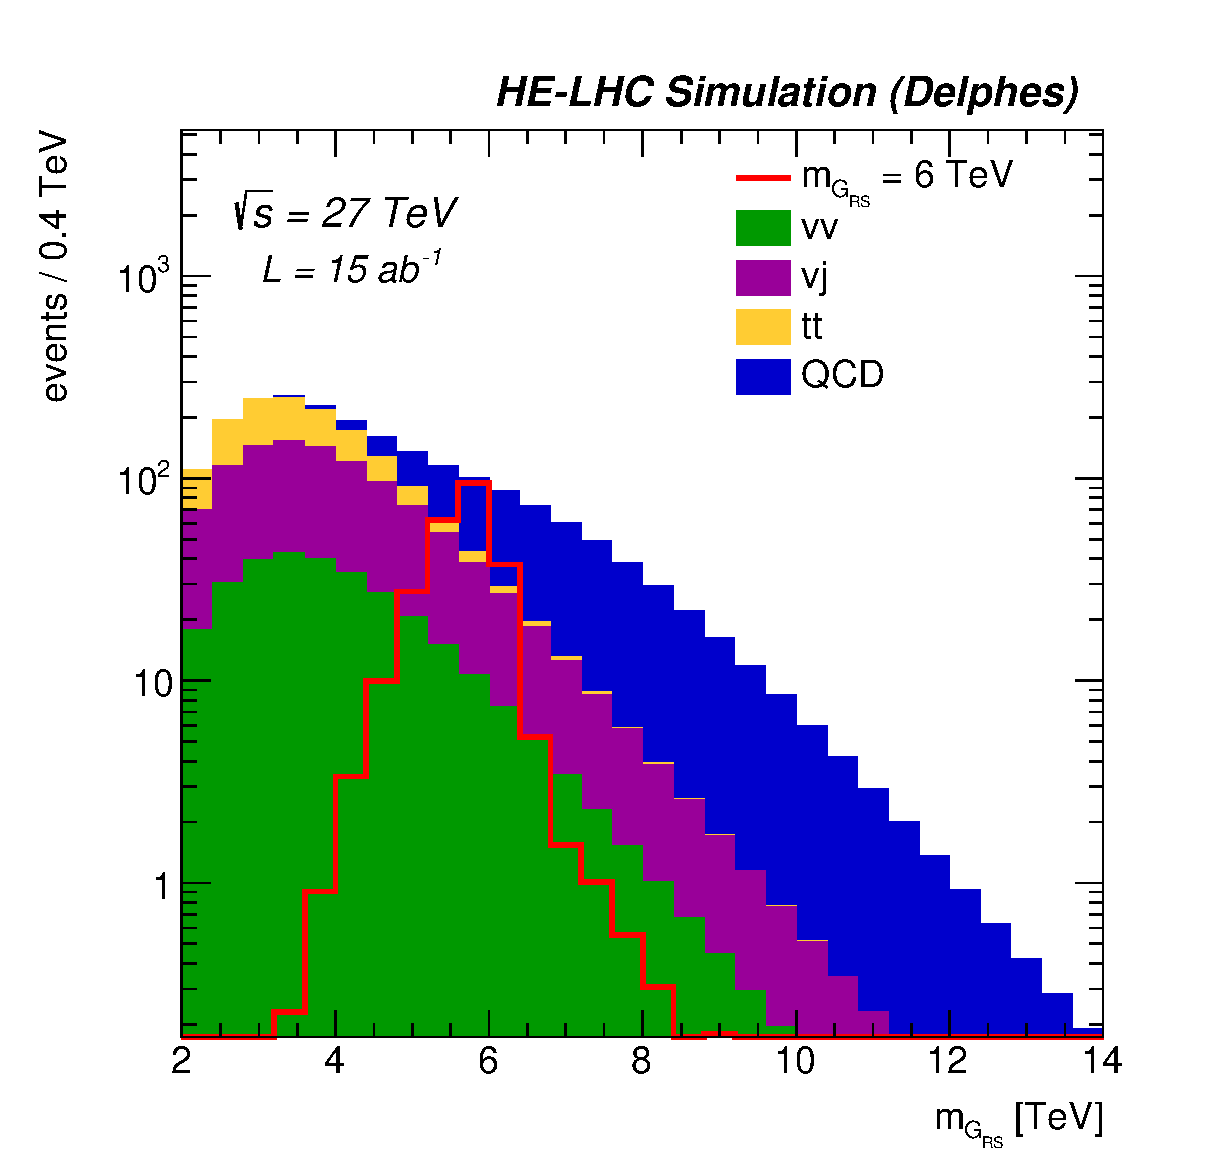
\includegraphics[width=0.30\columnwidth]{\main/section7OtherSignatures/img/RSGWW_Mj1j2_pf08_fit_sel4_nostack_log.eps}
  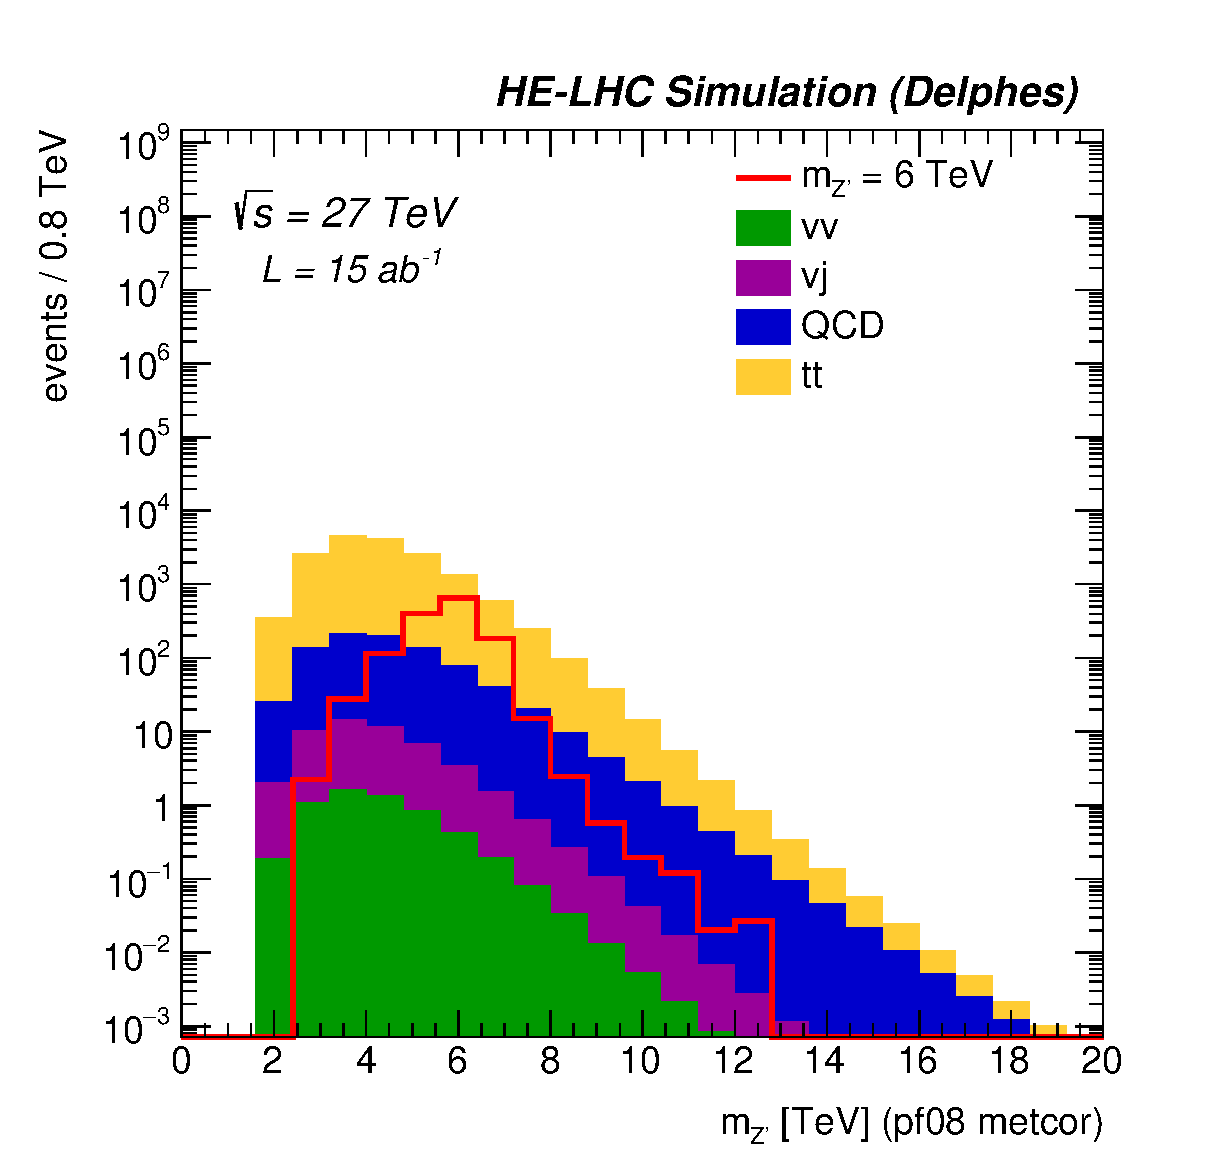
\includegraphics[width=0.30\columnwidth]{\main/section7OtherSignatures/img/Zptt_Mj1j2_pf08_MetCorr_fit_sel8_nostack_log.eps}
  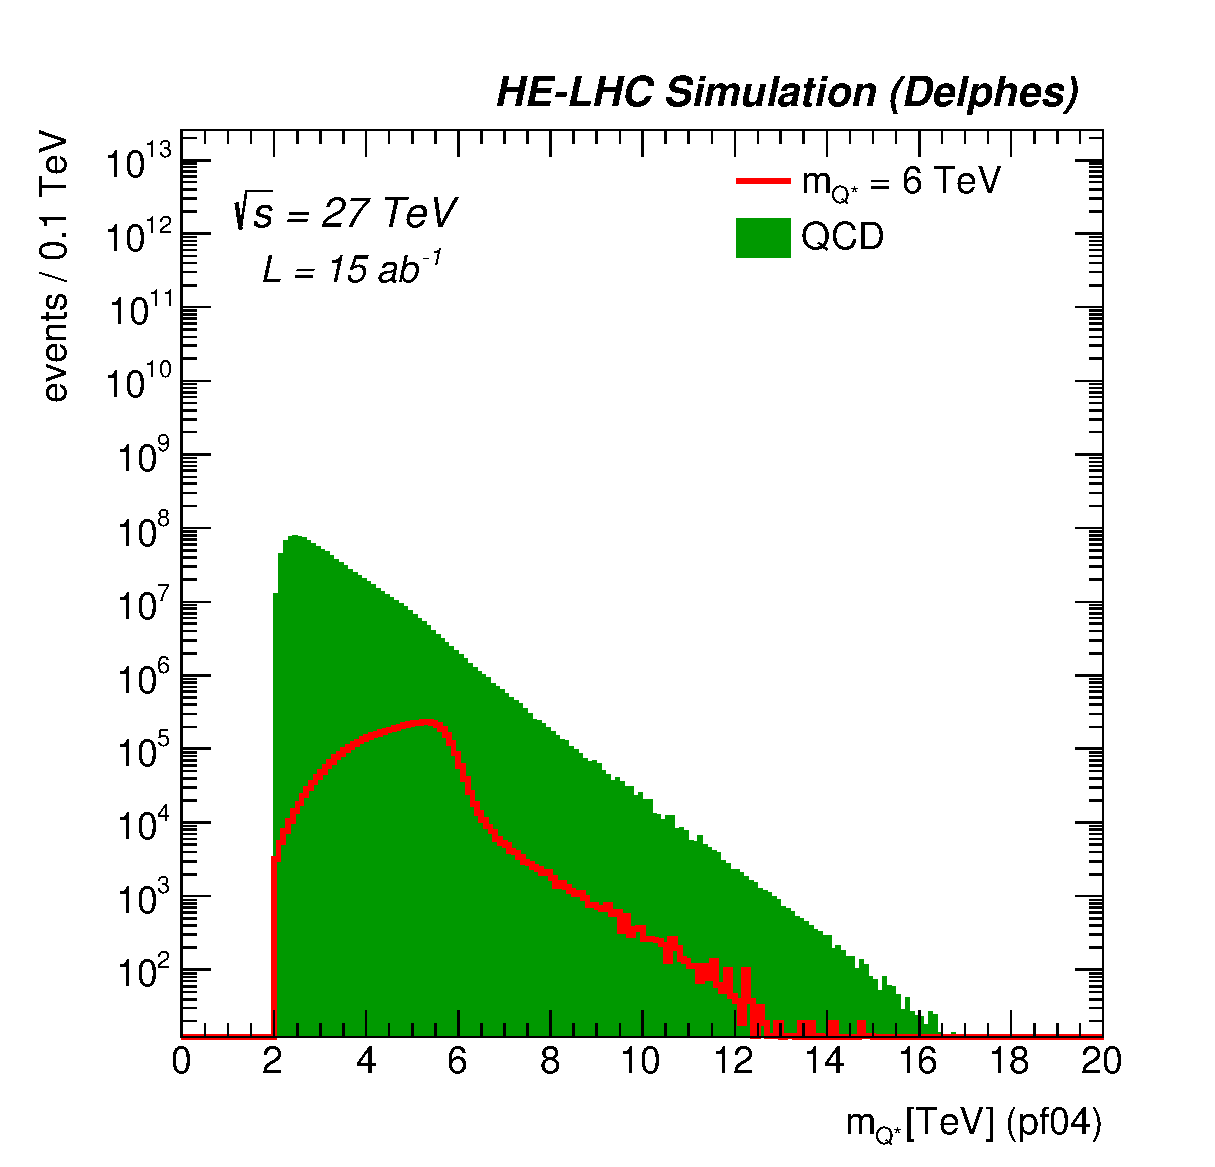
\includegraphics[width=0.30\columnwidth]{\main/section7OtherSignatures/img/qq_Mj1j2_pf04_sel1_nostack_log.eps}
  \caption{Invariant mass distribution of the two selected jets for the full selection for a 6~TeV signal for the three benchmark analyses  \zptt\ (left),  \rsg\ (center) and \qjj\ (right)}
  \label{fig:hadres_invmass}
\end{figure}

The event selection proceeds as follows:  we require two jets with $\pt>1$~TeV, $|\eta|<3$ and a small rapidity gap $\Delta\eta$~<~1.5 between the two high \pt\ jets. For the \zptt\ and \rsg\ searches, the rapidity gap selection is relaxed to $\Delta\eta$~<~2.4, both jets are required to be respectively top or $W$-tagged, and, to further reject background QCD jets, we require for both jets a large soft-dropped mass $m_\text{SD}>40$~GeV. Finally, for the \zptt\ search alone, we require that both selected jets must also be $b$-tagged. Since no lepton veto is applied, there is also some acceptance for leptonic decays. The sensitivity to semi-leptonic $\ttbar$ decays is enhanced by adding the $\metvec$ vector to the closest jet 4-momentum (among the two leading jets). The invariant mass of the two selected jets is used as a discriminant and is shown for the three benchmark analyses in Figure~\ref{fig:hadres_invmass}.


%%%%%%%%%%%%%%%%%%%%%%%%%%%%%%%%%%%%%%%%%%%%%%%%%%%%%%%%%%%%%%%%%%%%%%%%%%%%%%%%%%%%%%%%%%%%
%\subsubsection{Signal extraction and results}
%\paragraph*{Signal extraction and results}
Hypothesis testing is performed using a modified frequentist method based on a profile likelihood fit that takes into account the systematic uncertainties (mostly the background normalisations) as nuisance parameters. The expected exclusion limit at 95\%~\cl and discovery reach at 5~$\sigma$ are shown in Figures~\ref{fig:hadres_limits} (top and bottom) for the various scenarios that have been considered. At \sqrtshelhc, and with an integrated luminosity \intlumihelhc, it is possible to discover a $G_{RS}$ up to $m_{G}\approx~7$~TeV, and to exclude $m_{G}\lesssim~8$~TeV. For the \zptt\ search the exclusion reach is $m_{Z^{\prime}}\lesssim~10(8.5)$~TeV and it is possible to discover it up to $m_{Z^{\prime}}\approx 8(6.5)$~TeV for the TC2 and SSM models respectively. Finally, for the excited quark model, the exclusion reach is $m_{Q^{*}}\lesssim~$14TeV and the discovery reach is $m_{Q^{*}}\approx$~12TeV.

\begin{figure}[htbp]
  \centering
  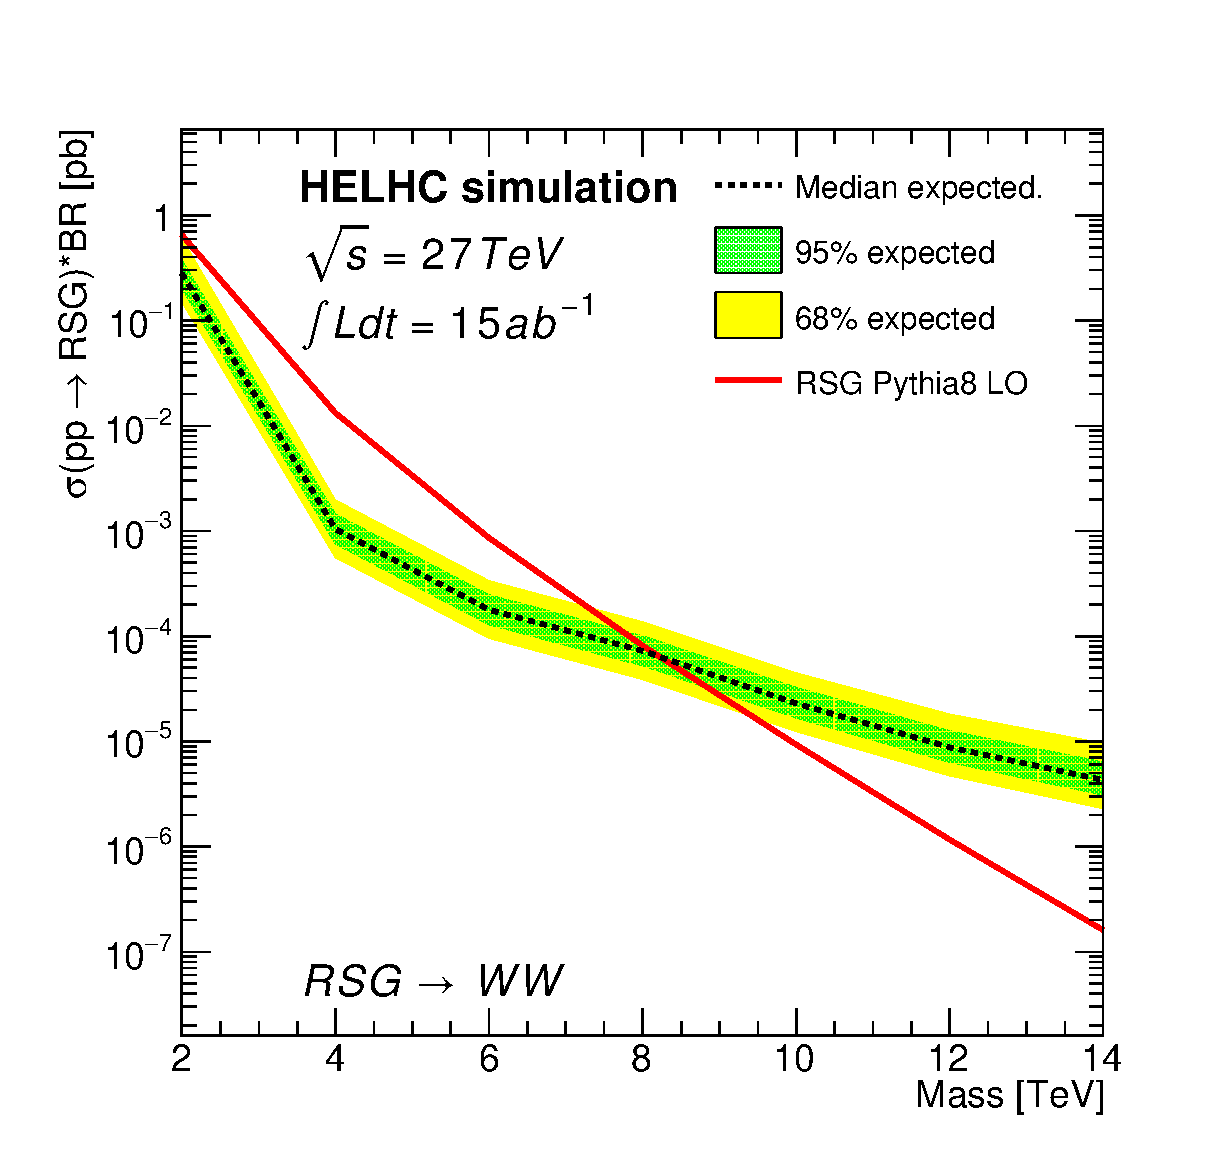
\includegraphics[width=0.30\columnwidth]{\main/section7OtherSignatures/img/lim_RSGraviton_ww_helhc_v01.eps}
  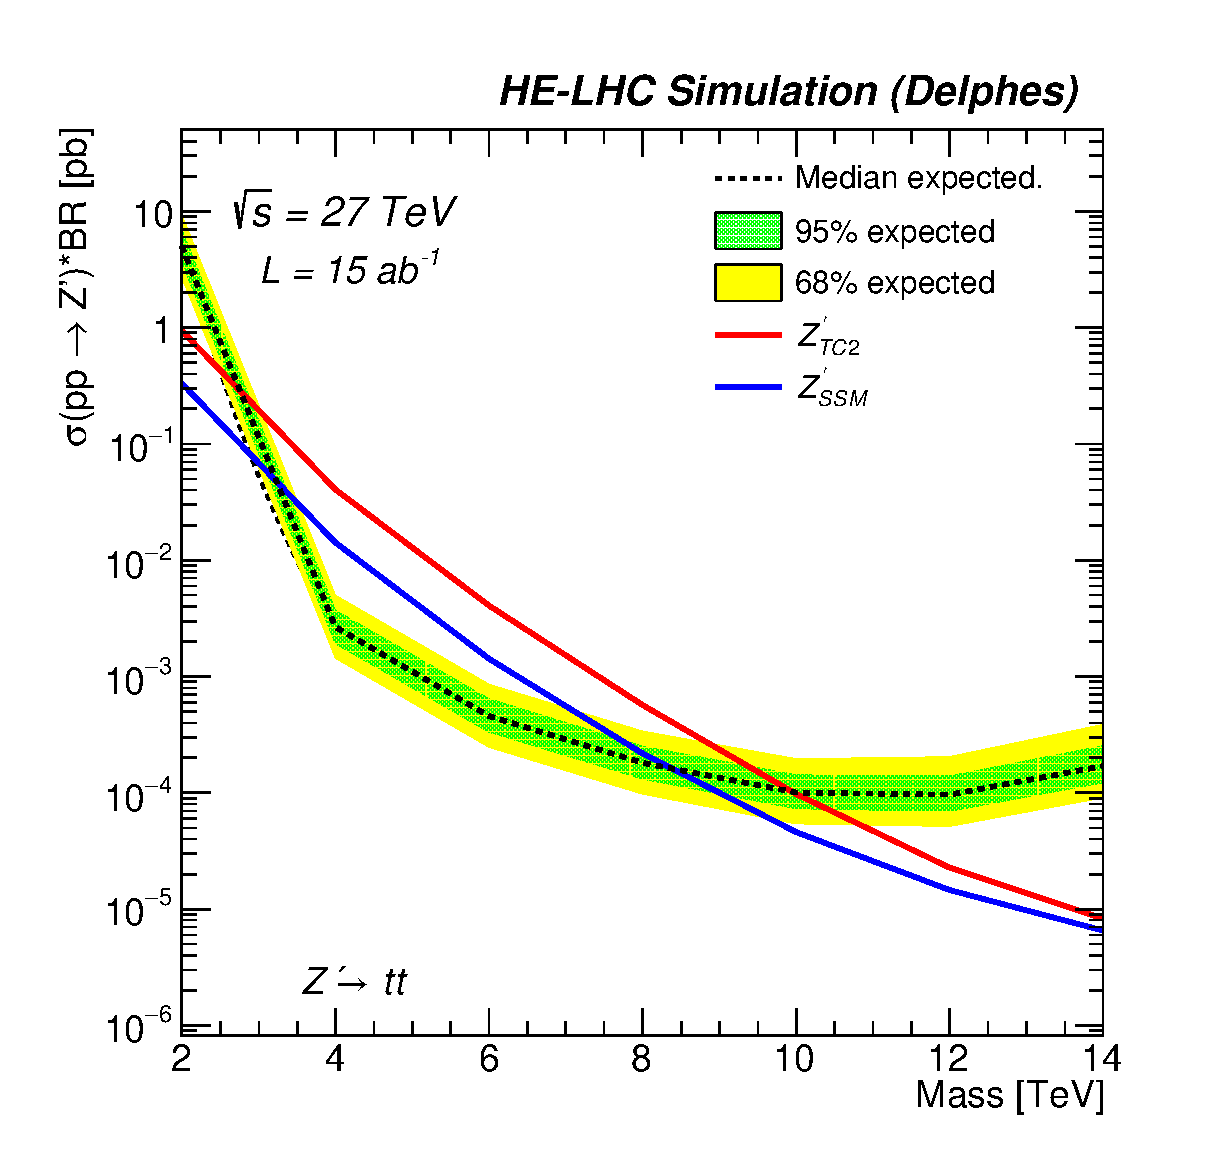
\includegraphics[width=0.30\columnwidth]{\main/section7OtherSignatures/img/lim_Zprime_tt_helhc_v01.eps}
  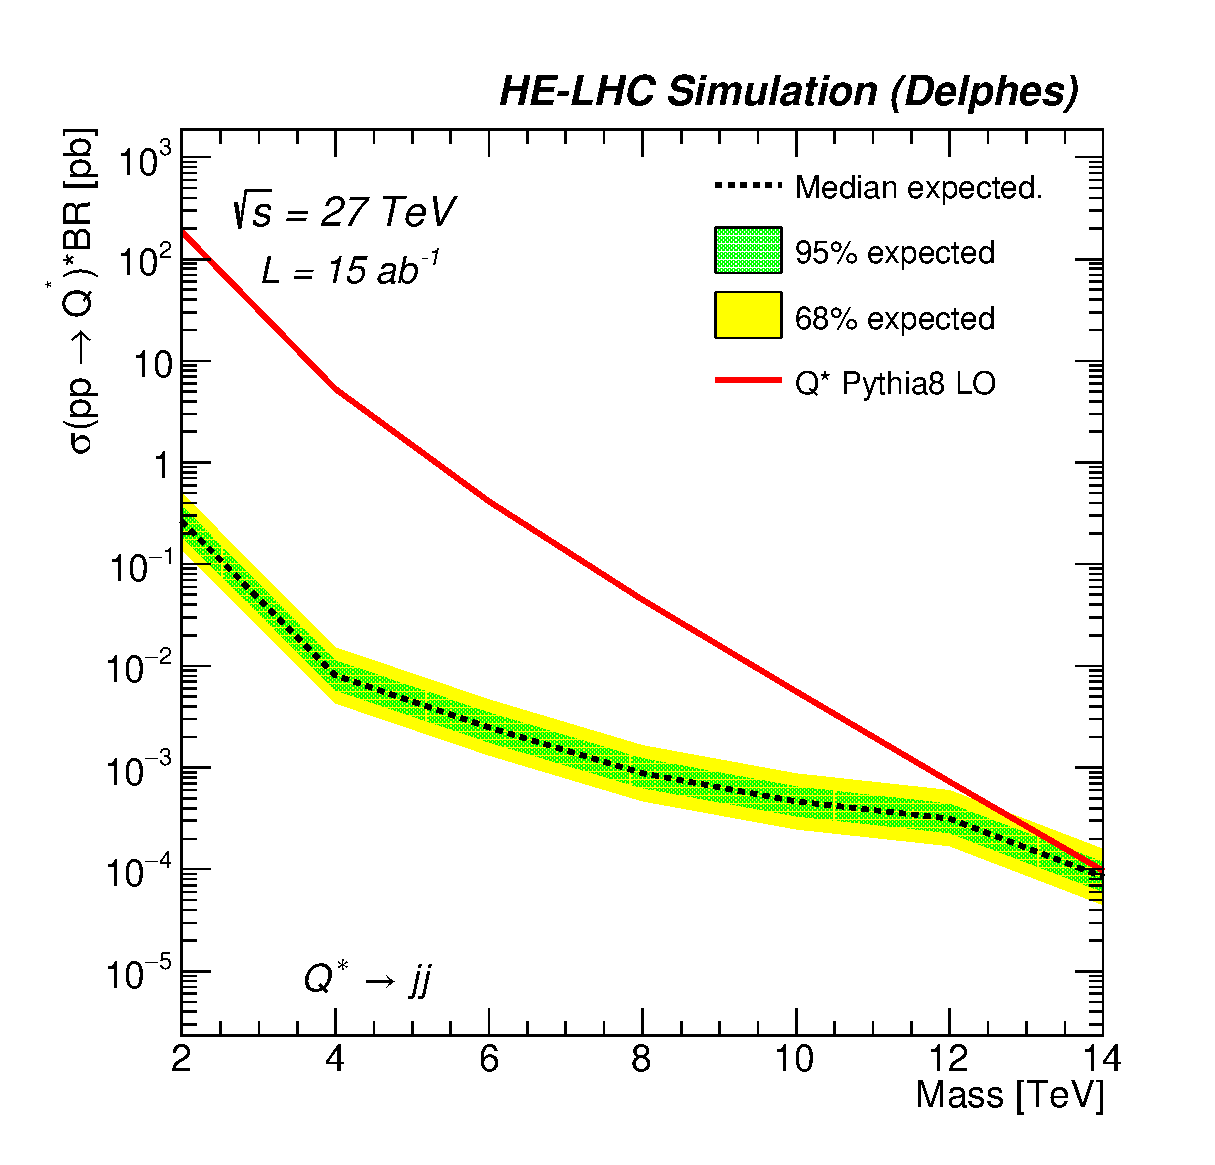
\includegraphics[width=0.30\columnwidth]{\main/section7OtherSignatures/img/lim_Qstar_jj_helhc_v01.eps}

  \includegraphics[width=0.30\columnwidth]{\main/section7OtherSignatures/img/DiscoveryPotential_ww_tagger_rootStyle.eps}
  \includegraphics[width=0.30\columnwidth]{\main/section7OtherSignatures/img/DiscoveryPotential_tt_SSM_TC2_tagger_TRFbtag_rootStyle.eps}
  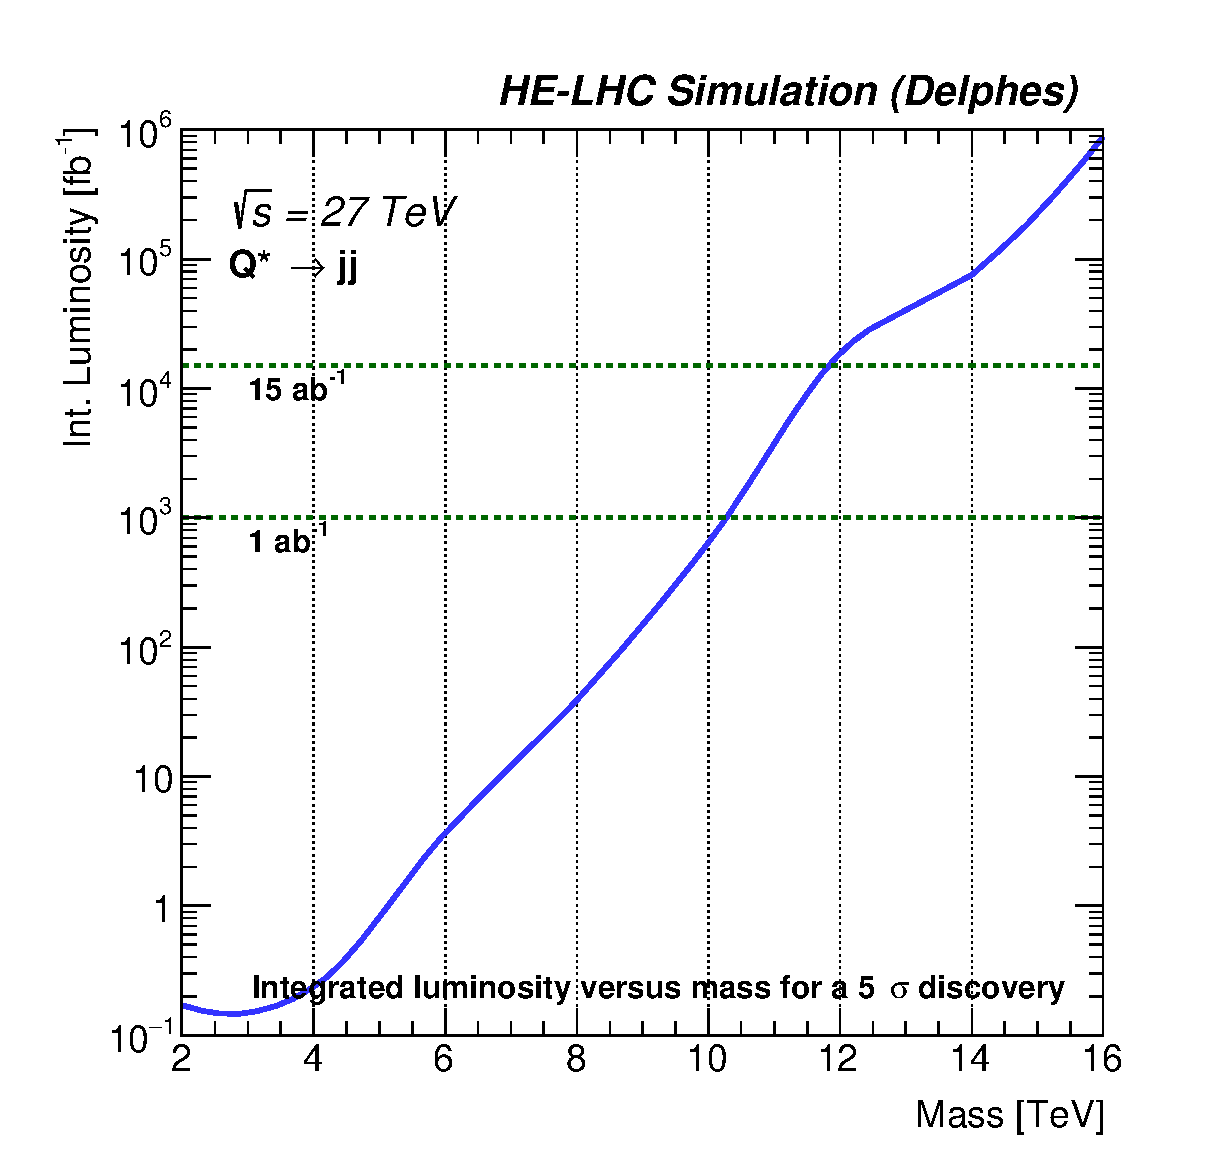
\includegraphics[width=0.30\columnwidth]{\main/section7OtherSignatures/img/DiscoveryPotential_jj_rootStyle.eps}

  \caption{Top: Exclusion limit at 95\%~\cl versus heavy resonance mass for the three benchmark models: \zptt\ (left),  \rsg\ (center) and \qjj\ (right). Bottom: Integrated luminosity needed for a $5\sigma$ discovery as a function of the heavy resonance mass for the three benchmark models.}
  \label{fig:hadres_limits}
\end{figure}

ADD FIGURE SUMMARY HELHC?
